\documentclass[12pt]{article}
\usepackage{latexsym}
\usepackage{amssymb,amsmath}
\usepackage[pdftex]{graphicx}
\usepackage{color}
\usepackage{hyperref}
\usepackage{epstopdf}


\topmargin = 0.1in \textwidth=5.7in \textheight=8.6in

\oddsidemargin = 0.2in \evensidemargin = 0.2in


\begin{document}\textsl{}

\begin{center}
COMPUTER SCIENCE 20, SPRING 2014 \\

Module \#18 (Digraphs and Relations)  - Checkin\\
Author: Tawheed Abdul-Raheem
\end{center}


\begin{enumerate}
\item Draw a directed graph with 3 vertices $A, B, C$ representing a relationship that is:
\begin{enumerate}
\item Reflexive
    \begin{center}
    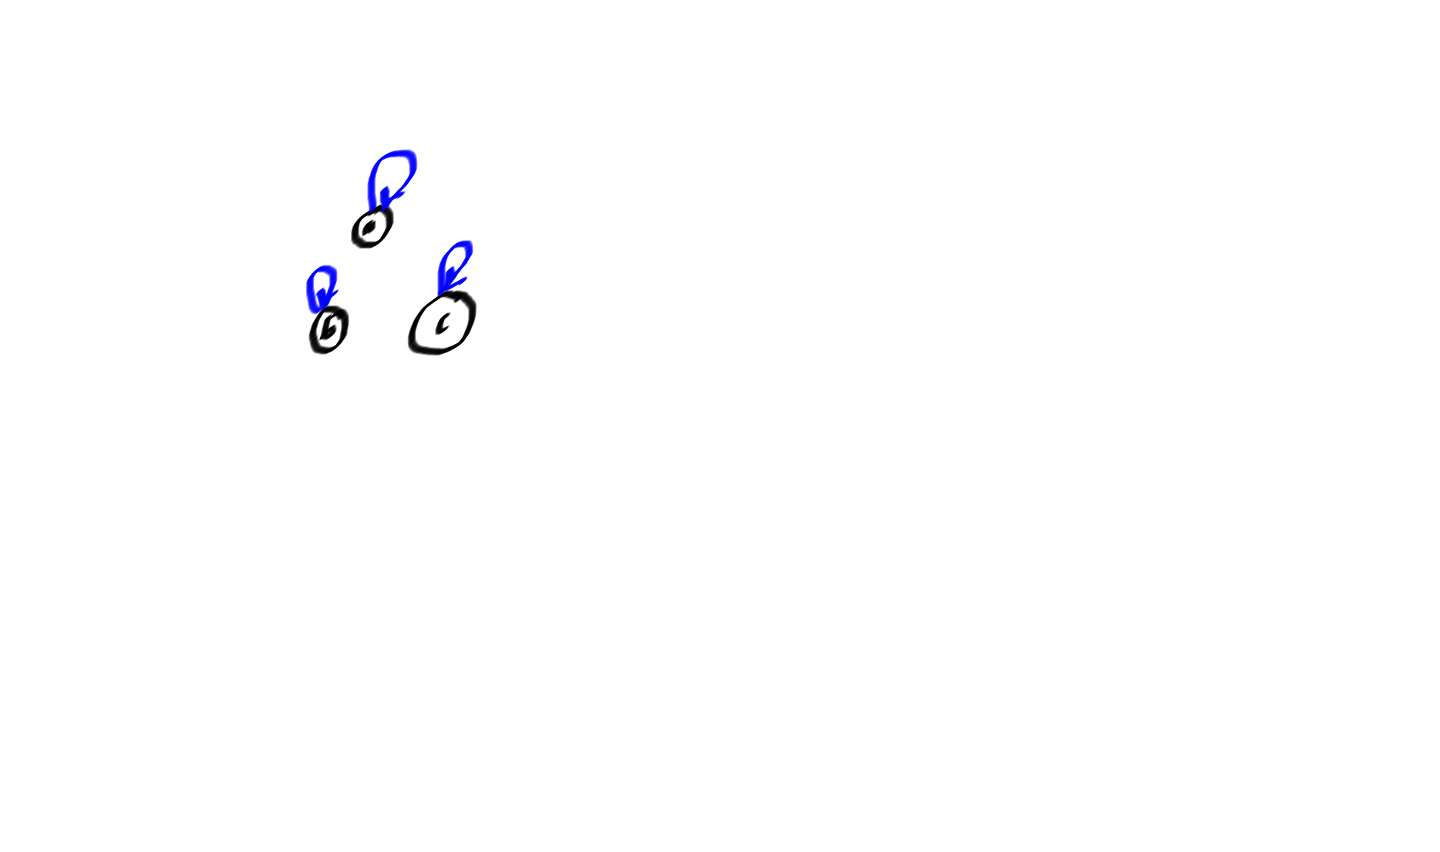
\includegraphics[scale=0.50]{reflexive.png}
    \end{center}
\item Symmetric
    \begin{center}
    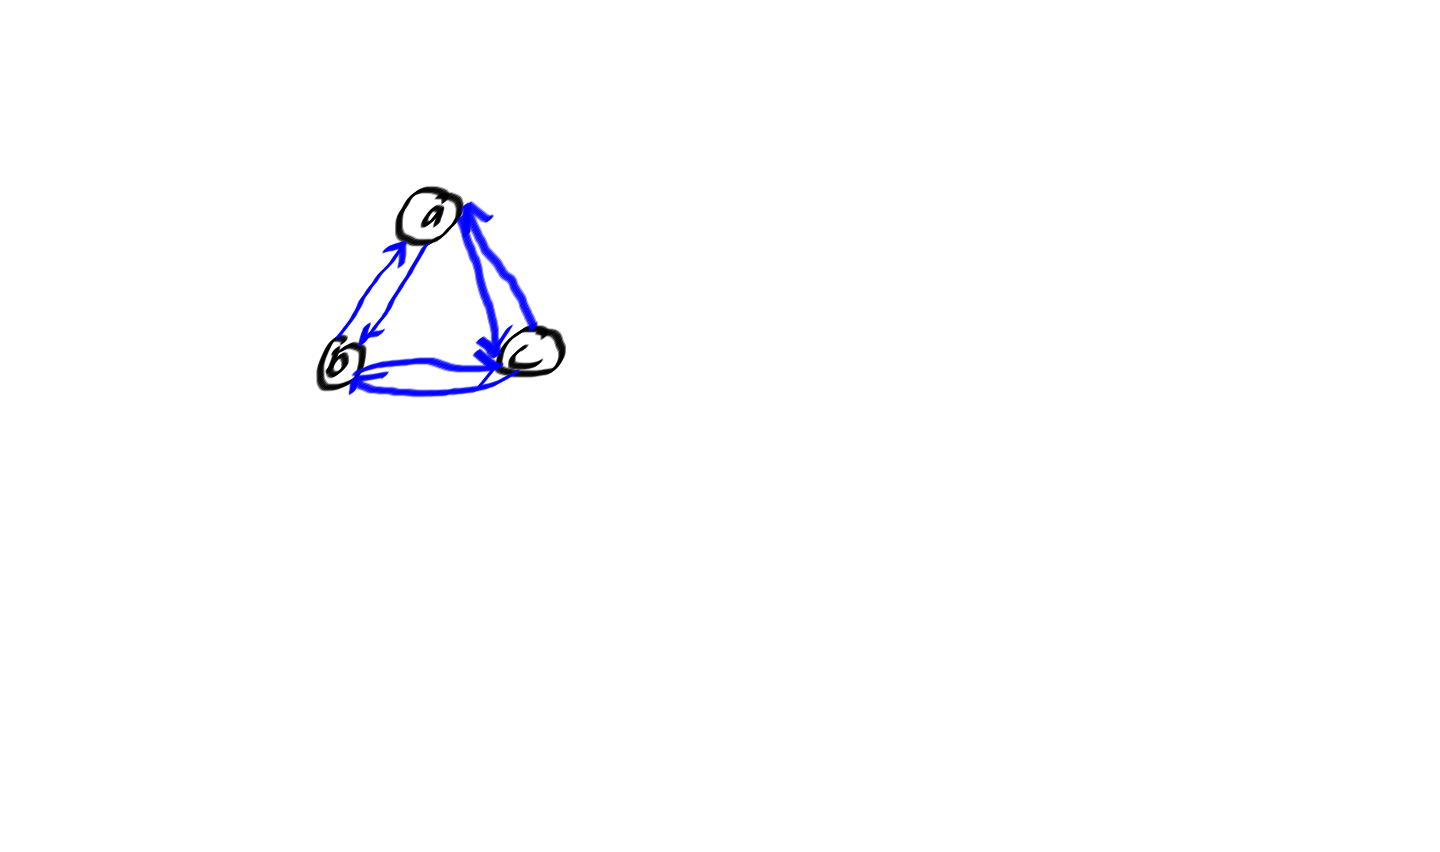
\includegraphics[scale=0.50]{symmetry.png}
    \end{center}
\item Antisymmetric
    \begin{center}
    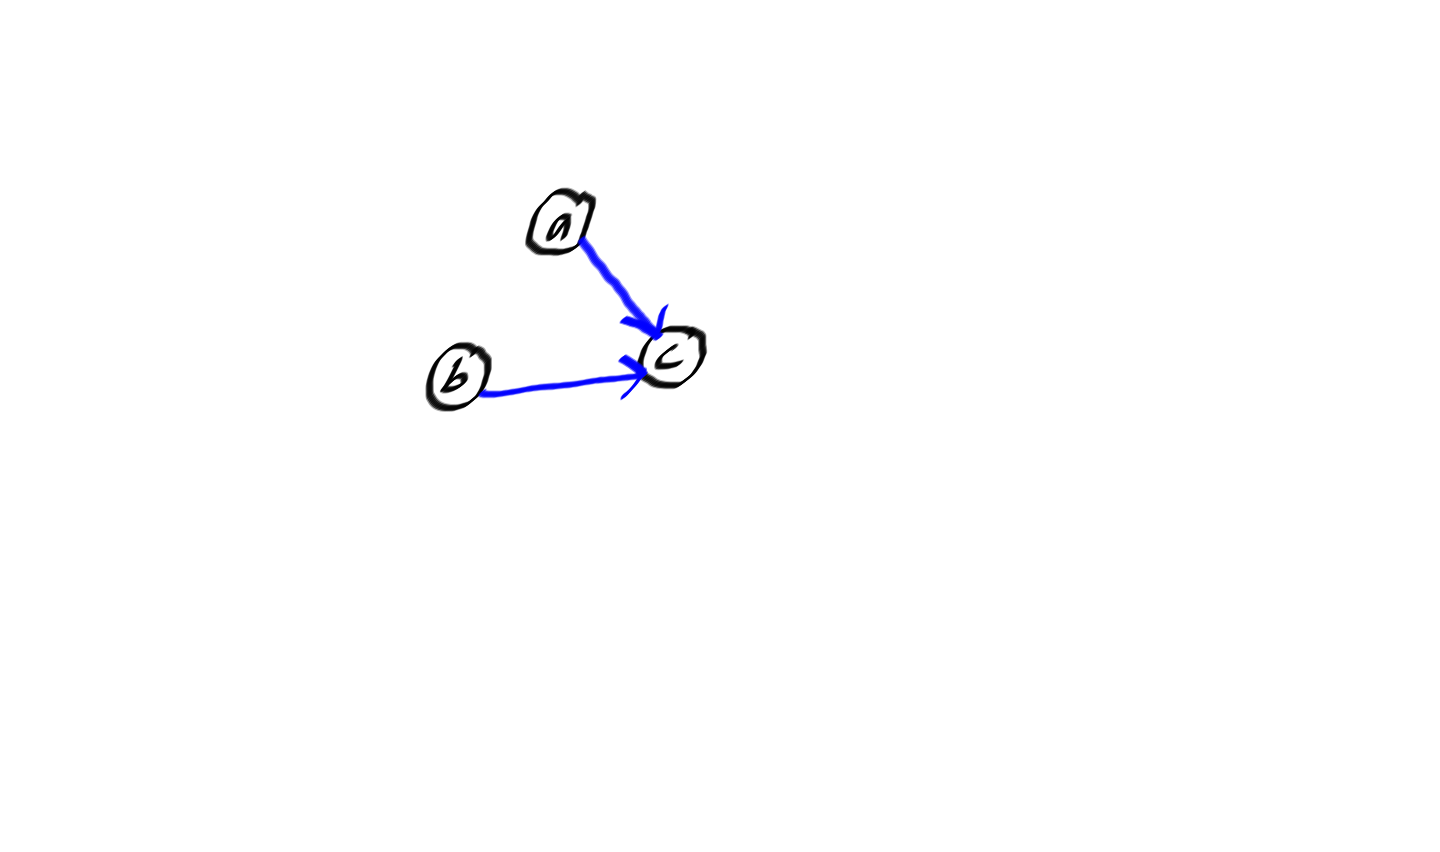
\includegraphics[scale=0.50]{antisymmerty.png}
    \end{center}
\item Transitive
    \begin{center}
    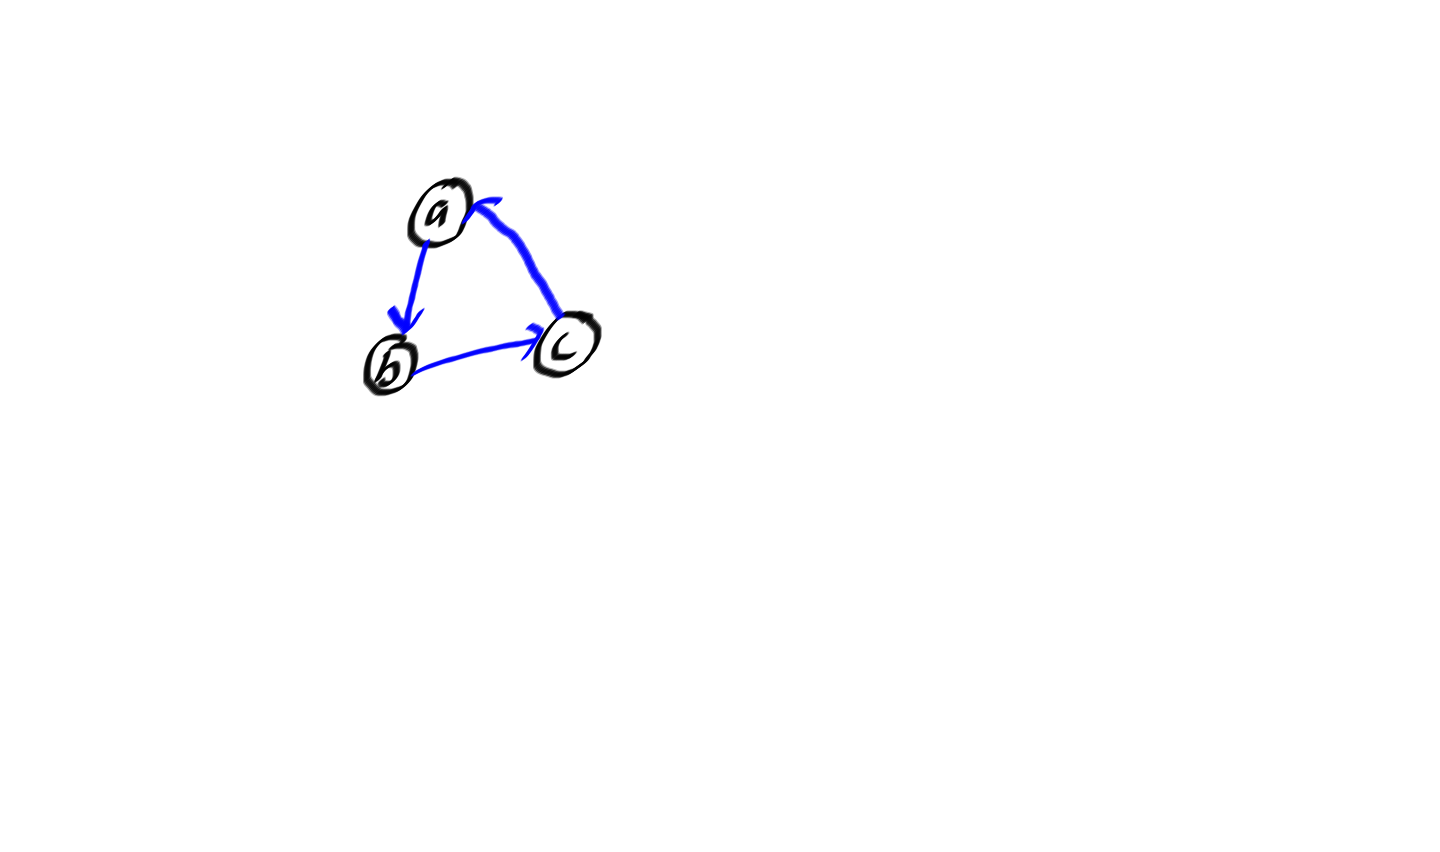
\includegraphics[scale=0.50]{transitive.png}
    \end{center}
\end{enumerate}
\end{enumerate}
\pagebreak


\end{document}

